\begin{figure}[H]
    \centering
    \includegraphics[width=.9\linewidth]{al_algo}
    \captionsetup{singlelinecheck=off}
    \caption[]{A Flowchart of the Algorithm
    \begin{description}
        \item[\protect{\parbox[t]{0.2\linewidth}{NN}}]
        \parbox[t]{0.8\linewidth}{convolutional neural ntwork trained to map spectra to stack and layer \\ parameters}
        \item[\protect{\parbox[t]{0.2\linewidth}{DB}}]
        \parbox[t]{0.8\linewidth}{database of FMM simulated single layers}
        \item[\protect{\parbox[t]{0.2\linewidth}{SASA}}]
        \parbox[t]{0.8\linewidth}{algorithm calculating $\hat{S}_\s{stack} = \hat{S}_\s{stack}(\hat{S}_1, \, \hat{S}_2, \, ...)$}
        \item[\protect{\parbox[t]{0.2\linewidth}{Opt}}]
        \parbox[t]{0.8\linewidth}{optimizer changing parameters to minimize the difference between the current and target spectrum}
        \item[\protect{\parbox[t]{0.2\linewidth}{$\bm{\hat{S}_1}, \, \bm{\hat{S}_2}$}}]
        \parbox[t]{0.8\linewidth}{S-matrices of the top and bottom layer}
        \item[\protect{\parbox[t]{0.2\linewidth}{layer\\params}}]
        \parbox[t]{0.8\linewidth}{these include the geometry of the periodic meta surface cell and the kind of material used}
        \item[\protect{\parbox[t]{0.2\linewidth}{stack\\params}}]
        \parbox[t]{0.8\linewidth}{the rotation angle of the layers to one another and the distance between}
        \item[\protect{\parbox[t]{0.2\linewidth}{new\\params}}]
        \parbox[t]{0.8\linewidth}{the Opt. only changes the continuous parameters, the discrete ones , e.g. material, remain unchanged}
        \item[\protect{\parbox[t]{0.2\linewidth}{optimization\\loop}}]
        \parbox[t]{0.8\linewidth}{this loop is repeated until the target accuracy is reached}
    \end{description}}
    \label{fig:al:algo}
\end{figure}

\subsection{Network}
\subsection{Database}
\subsection{Optimizer}
